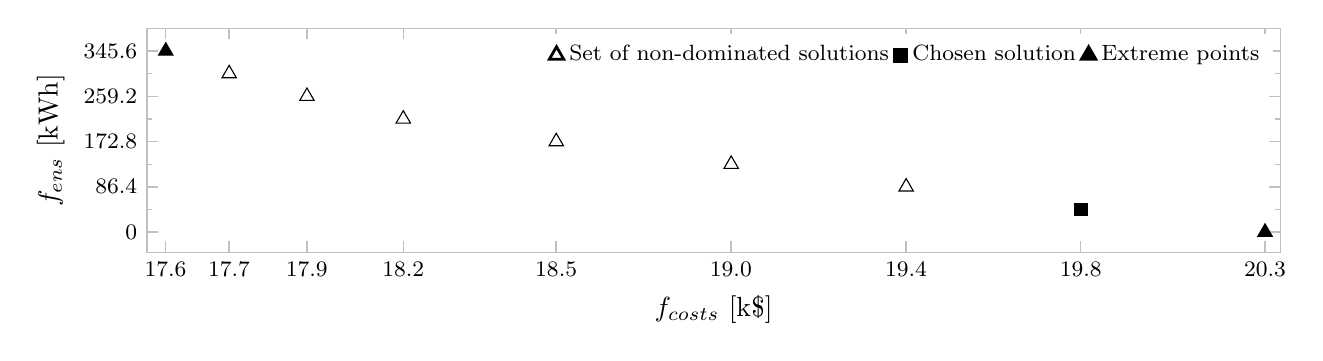
\begin{tikzpicture}
    \begin{axis}[
        %width=240pt,
        % height = 140pt,
        % x dir = reverse,
        y post scale = 0.5,
        x post scale = 2.1,
        xlabel={$f_{costs}$ [k\$]},
        xlabel near ticks,
        % axis x line = bottom,
        % axis line shift = 10pt,
        ylabel={$f_{ens}$ [kWh]},
        ylabel near ticks,
        % axis y line = left,
        % axis line style={|-stealth},
        % axis x discontinuity=crunch,
        tick style = {line width = 0.5, color = lightgray, 
            major tick length=4pt,minor tick length=2pt, 
            minor y tick num =1, xtick = {
            17645, 
            17799,
            17988,
            18222,
            18593,
            19017,
            19442,
            19866,
            20313}
            },
        xticklabels = {
            17.6,
            17.7,
            17.9,
            18.2,
            18.5,
            19.0,
            19.4,
            19.8,
            20.3
            },
        tick label style = {font=\footnotesize, ytick distance=86.4
            },
        xtick align = {inside},
        ytick align = {inside},
        % extra x ticks={10926.93},
        %extra x tick labels={10926.93},
        % label style = {font=\small},
        % legend style = {font=\footnotesize, at={(0.5,1.05)},    
        %     anchor=south, legend cell align=left, line width=0.5pt, 
        %     draw=lightgray, legend columns = 2}
        legend style = {font=\footnotesize, at={(0.995,0.98)},    
            anchor= north east, legend cell align=center, line width=1pt, 
            draw = none, legend columns = 3},
        ymax=388.8,
        xmin=17600, xmax=20350,
        % enlarge x limits=0.05,
        axis line style = {line width = 0.5pt, lightgray},
        scaled ticks=false
        ]

    
     % Set of non-dominated solutions 
    \addplot[mark = triangle, only marks, mark size = 3pt,
    black] 
    coordinates {

        (17799.57	,302.4)
        (17988.30	,259.2)
        (18222.13	,216)
        (18593.29	,172.8)
        (19017.81	,129.6)
        (19442.34	,86.4)
        % (19866.86	,43.2)
              
        };
    \addlegendentry{Set of non-dominated solutions}
    
    % Centroid
    \addplot [mark size = 2.2pt, only marks, mark = square*]
        coordinates {
        (19866.86	,43.2)
        };
    \addlegendentry{Chosen solution}

    \addplot [mark size = 3pt, only marks, mark = triangle*]
        coordinates {
        (17645.70	,345.6)
        (20313.20	,0)
        };
    \addlegendentry{Extreme points}
    % \node [coordinate, pin=above right:{Centroid}] at
    %     (axis cs: 13863.73, 259.2 ) {};
    % \node [coordinate, pin=above right:{Ideal Point}] at
    %     (axis cs: 10926.93, 0) {};
    \end{axis}
\end{tikzpicture}